% !TeX spellcheck = en_US
% Chapter 1

%\chapter{Chapter Title Here} % Main chapter title
%
%\label{Chapter1} % For referencing the chapter elsewhere, use \ref{Chapter1} 

%----------------------------------------------------------------------------------------

% Define some commands to keep the formatting separated from the content
%\newcommand{\option}[1]{\texttt{\itshape#1}}

%----------------------------------------------------------------------------------------
\chapter{Spherical study}
	\section{Setup}
		The host galaxy has two mass distributions that are superimposed, one for dark matter and the other one for all the luminous or baryonic matter.
		\begin{figure}[h]
			\centering
			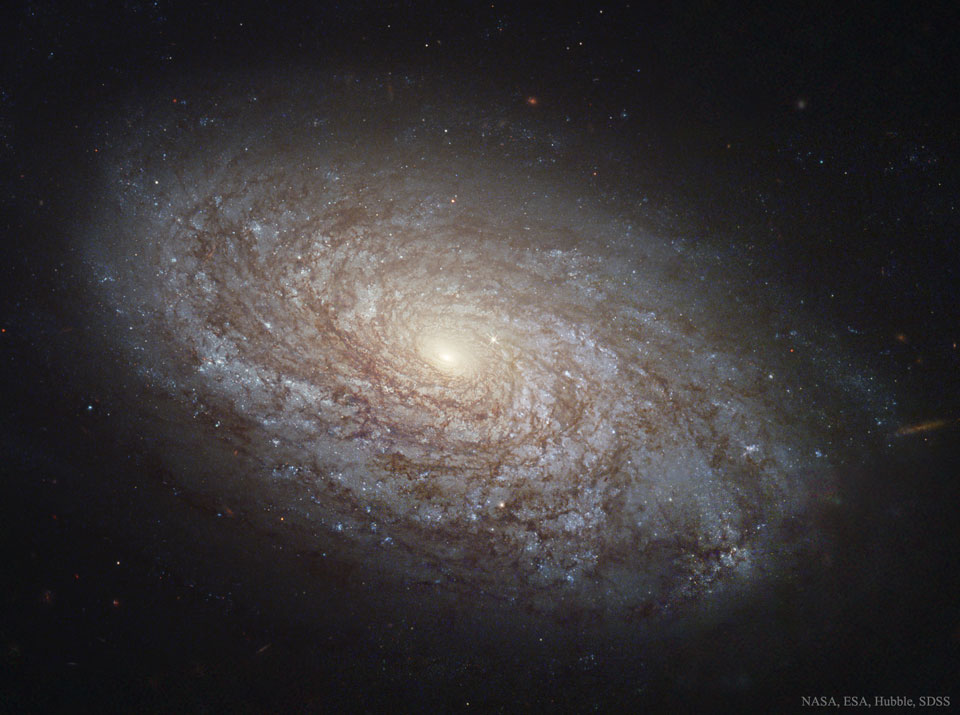
\includegraphics[width=0.8\linewidth]{Figures/NGC4414_modified}
			\caption{NGC4414 galaxy as seen by the Hubble telescope.}
		\end{figure}
	
		The dark matter halo used, follows a NFW (Navarro–Frenk–White) profile, baryonic matter is divided in stars and gas, for gas a power law profile with $r^{-2.2}$ is used, while for stars a Hernquist model is applied \cite{tanaka2009assembly, choksi2017recoiling}. The sum of all these components accounts for the total mass of the host ($M_h$), which remains constant through a simulation. The amount of baryonic matter is given by the baryonic fraction parameter ($f_b$), and the mass of stars by the stellar fraction parameter ($f_s$). Cumulative masses at the virial radius are defined as follows:
		\begin{equation}
			M_\text{DM}(R_\text{vir}) = (1 - f_b)M_h
		\end{equation}
		\begin{equation}
			M_\text{stars}(R_\text{vir}) = f_sf_bM_h
		\end{equation}
		\begin{equation}
			M_\text{gas}(R_\text{vir}) = (1 - f_s)f_bM_h
		\end{equation}
		
	\subsection{Virial radius}
		Since all of the density profiles are spherically symmetrical, it follows from \autoref{eq: R_vir_def} that:  
		\begin{equation}
			\dfrac{M_h}{4/3\pi R_\text{vir}^3} = 75\dfrac{H(t)^2}{\pi G}
		\end{equation}
		\begin{equation}
			R_\text{vir} = \left({\dfrac{M_hG}{100 H(t)^2}}\right)^{1/3}
		\end{equation}
	
	\subsection{Dark matter halo}
		For a dark matter halo following a NFW profile, the density at some distance $r$ is given by the formula:
		\begin{equation}\label{eq: dmdensity}
			\rho_\text{DM}(r) = \dfrac{\rho_0^\text{DM}}{\frac{r}{R_s}\left(1 + \frac{r}{R_s}\right)^2}
		\end{equation}
		
		Where $R_s$ and $\rho_0^\text{DM}$ are constants for a given dark matter halo. Using the density, the cumulative mass $M_\text{DM}(r)$ within some radius $r$ is given by the integral of the density over a volume, since \autoref{eq: dmdensity} is spherically symmetrical, the only dependance of the integral is with distance. On \autoref{eq: cumulativeDM} the $r'^2$ comes from the Jacobian of spherical coordinates, and the $4\pi$ from the solid angle.
		\begin{equation}\label{eq: cumulativeDM}
			M_{DM}(r) = \int\limits_0^{r} 4\pi {r'}^2\rho_\text{DM}(r')dr' = 4\pi\rho_0^\text{DM}R_s^3\left[\ln\left(\dfrac{R_s + r}{R_s}\right) - \dfrac{r}{R_s + r}\right]
		\end{equation}
		
		Considering a concentration parameter $c(M_h, z)$ of dark matter in the halo, the following relation holds for the viral radius $R_\text{vir}$ and the scale radius $R_s$:
		\begin{equation}\label{eq: virialConcentration}
			R_\text{vir} = c(M_h, z)R_s
		\end{equation}
		
		Where the concentration parameter, dependence with the dark matter halo mass ($M_h$) and redshift is given by: 
		\begin{equation}
			c(M_h, z) = c_0(z)\left(\dfrac{M_h}{10^{13}M_\theta}\right)^{\alpha(z)}
		\end{equation}
		
		where $\alpha(z)$ and $c_0(z)$ were fitted using simulation data to the following functions \cite{choksi2017recoiling}:
		\begin{equation}
			c_0(z) = \dfrac{4.58}{2}\left[\left(\dfrac{1 + z}{2.24}\right)^{0.107} + \left(\dfrac{1 + z}{2.24}\right)^{-1.29}\right]
		\end{equation}
		
		\begin{equation}
			\alpha(z) = -0.0965 \exp\left(-\dfrac{z}{4.06}\right)
		\end{equation}
	
		\begin{figure}[h]
			\centering
			\includegraphics[width=0.7\linewidth]{"../Files/Week 3/darkmatter_concentration"}
			\caption{Dark matter concentration parameter as a function of the halo mass and the redshift.}
			\label{fig: dmconcentration}
		\end{figure}
	
		For a fixed halo mass, as time passes (smaller redshift), concentration of dark matter will increase, as can be shown on \autoref{fig: dmconcentration}, nevertheless for high redshifts concentration is approximately constant at $c \approx 3$ for all halos \cite{choksi2017recoiling}. By using \autoref{eq: virialConcentration} one can obtain the value of $\rho_0^\text{DM}$ by evaluating \autoref{eq: cumulativeDM} at $R_\text{vir}$.
		\begin{equation}\label{eq: dmM_virial}
			M_\text{DM}(R_\text{vir}) = 4\pi\rho_0^\text{DM}R_s^3 \left[\ln\left(\dfrac{R_s + c(M_h, z)R_s}{R_s}\right) - \dfrac{c(M_h, z)R_s}{R_s + c(M_h, z)R_s}\right] = (1 - f_b)M_h
		\end{equation}
		\begin{equation}\label{eq: rho0dm}
			\rho_0^\text{DM} = \dfrac{(1 - f_b)M_h}{4\pi \left(\dfrac{R_\text{vir}}{c(M_h, z)}\right)^3 \left[\ln\left(1 + c(M_h, z)\right) - \dfrac{c(M_h, z)}{1 + c(M_h, z)}\right]}
		\end{equation}
	
		\subsection{Stellar profile}
			Stellar density is modeled as a Hernquist profile with half-mass radius $R_{1/2} = 0.01 R_\text{vir}$, as in \citeauthor{choksi2017recoiling}. Density for a Hernquist profile is given by \cite{hernquist1990analytical}:
			\begin{equation}
				\rho_s(r) = \dfrac{f_sf_bM_h \mathcal{R}_s}{2\pi r(r + \mathcal{R}_s)^3} \qquad \text{$\mathcal{R}_s$ is known as scale length}
			\end{equation}
			
			Integrating from $0$ to $r$ yields:
			\begin{equation}
				M_s(r) = \dfrac{f_sf_bM_h r^2}{(r + \mathcal{R}_s)^2}
			\end{equation}
			
			The half-mass radius, as the name implies, is the distance at which the cumulative mass is half the total mass \cite{hernquist1990analytical}.
			\begin{equation}
				R_{1/2} = \left(1 + \sqrt{2}\right)\mathcal{R}_s = 0.01\left({\dfrac{M_hG}{100 H(t)^2}}\right)^{1/3}
			\end{equation}
			
			From which the scale length can be set as a function of the time when the kick occurs, and the mass of the host, as:
			\begin{equation}
				\mathcal{R}_s = \dfrac{0.01}{\left(1 + \sqrt{2}\right)}\left({\dfrac{M_hG}{100 H(t)^2}}\right)^{1/3} \approx 6.835\times 10^{-4}\left({\dfrac{M_h}{H(t)^2}}\right)^{1/3}
			\end{equation}
	
		\subsection{Gas profile}
			For high redshift the baryonic profile resembles that of a gaseous galaxy, \citeauthor{choksi2017recoiling} use a constant density gas core of $r_0 = 1$ pc, followed by a power law of $r^n = r^{-2.2}$. The complete density is described as follows:
			\begin{equation}
				\rho_\text{gas}(r) = \left \{
					\begin{matrix}
					\rho_0^\text{gas} & \text{if $r < r_0$}\\
					\rho_0^\text{gas}\left(\dfrac{r_0}{r}\right)^{-n} & \text{if $r \geq r_0$}\\
					\end{matrix}
				\right.
			\end{equation}
			
			The cumulative mass is found by integrating the density in spherical coordinates, which for $n \neq -3$ is equal to:
			\begin{equation}
				M_\text{gas}(r) = \left \{
					\begin{matrix}
					\dfrac{4}{3}\pi\rho_0^\text{gas}r^3 & \text{if $r < r_0$} \\
					4\pi\rho_0^\text{gas}\left(\dfrac{\left(r^{3 + n} - r_0^{3 + n}\right)}{(3+n)r_0^{n}}  + \dfrac{r_0^3}{3}\right) & \text{if $r \geq r_0$} \\
					\end{matrix}
				\right.
			\end{equation}
			
			The value of the constant $\rho_0^\text{gas}$ is found using a similar process as in \autoref{eq: dmM_virial} and \ref{eq: rho0dm}.
			\begin{equation}
				M_\text{gas}(R_\text{vir}) = 4\pi\rho_0^\text{gas}\left(\dfrac{\left(R_\text{vir}^{3 + n} - r_0^{3 + n}\right)}{(3+n)r_0^{n}} + \dfrac{r_0^3}{3}\right) = (1 - f_s) f_bM_h
			\end{equation}
			\begin{equation}
				\rho_0^\text{gas} = \dfrac{(1 - f_s) f_bM_h}{4\pi \left(\dfrac{\left(R_\text{vir}^{3 + n} - r_0^{3 + n}\right)}{(3+n)r_0^{n}} + \dfrac{r_0^3}{3}\right)} = \qquad \text{ if $R_\text{vir} > r_0$}
			\end{equation}
			
			All of the profiles are shown on \autoref{fig: massprofiles}, where the effect of the stellar fraction can be seen.
			\begin{figure}[h]
				\centering
				\begin{subfigure}[b]{0.49\textwidth}
					\includegraphics[width=\textwidth]{"../Files/Week 6/density_mass_fs01"}
					\caption{Stellar fraction $f_s = 0.01$.}
					\label{fig: baryonicprofilehigh}
				\end{subfigure}
				~ 
				\begin{subfigure}[b]{0.49\textwidth}
					\includegraphics[width=\textwidth]{"../Files/Week 6/density_mass_fs3"}
					\caption{Stellar fraction $f_s = 0.30$.}
					\label{fig: baryonicprofilelow}
				\end{subfigure}
				\caption{Mass distributions for $R_\text{vir} = 0.69$ kpc (red line), $c = 4$, and $f_b = 0.156$.}
				\label{fig: massprofiles}
			\end{figure}
		
	\section{Effect of the baryonic fraction}
	
	\section{Effect of the power law exponent}
	
	\section{Effect of the stellar fraction}
	
%	\begin{figure}[h]
%		\centering
%		\includegraphics[width=\textwidth]{"../Files/Week 5/stellar_density_comparison"}
%	\end{figure}
%
%	\begin{figure}[h]
%		\centering
%		\includegraphics[width=0.7\textwidth]{"../Files/Week 5/properties_s02v70"}
%	\end{figure}
%	